% Figure 11 -- Riemann surface with regular and irregular punctures
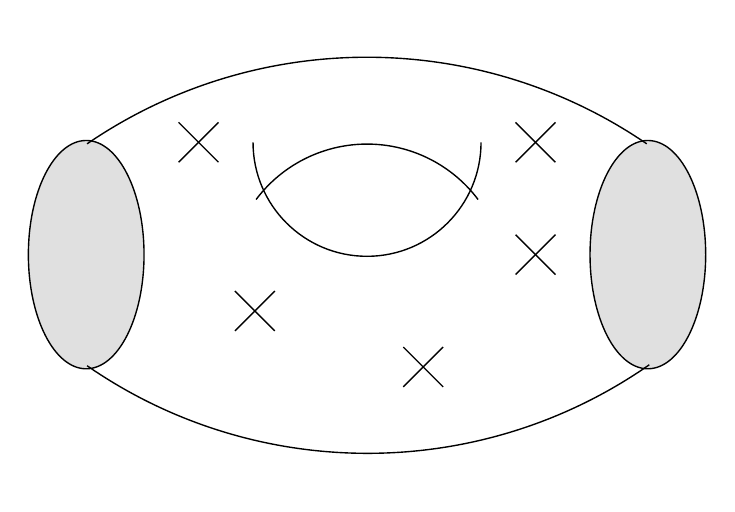
\begin{tikzpicture}[x=1pt,y=1pt,scale=1.10,transform shape,>=stealth,line width=0.5pt]
  \def\cr#1#2{\draw (#1-6.55,#2-6.55) -- (#1+6.55,#2+6.55);
               \draw (#1-6.55,#2+6.55) -- (#1+6.55,#2-6.55);}
  % ---- the two ends of the surface ----
  \draw[fill=black!12] (25.1,85.5) ellipse[x radius=19pt,y radius=37.5pt];
  \draw[fill=black!12] (209.6,85.5) ellipse[x radius=19pt,y radius=37.5pt];
  % ---- upper and lower boundary ----
  \draw (25.4,121.9) arc[start angle=124.4,end angle=55.6,radius=162.7pt];
  \draw (25.4,49.0) arc[start angle=235.3,end angle=304.9,radius=161.8pt];
  % ---- the cycle drawn on the surface ----
  \draw (80.9,103.6) arc[start angle=143.1,end angle=36.9,radius=45.6pt];
  \draw (79.9,122.4) arc[start angle=180,end angle=360,radius=37.45pt];
  % ---- punctures ----
  \cr{62.0}{122.4}
  \cr{172.7}{122.4}
  \cr{172.7}{85.5}
  \cr{80.5}{67.0}
  \cr{135.8}{48.6}
\end{tikzpicture}
